\documentclass[12pt,a4paper]{article}

%-------------------Packages-------------------%
\input Acorn.fd
\usepackage[magyar]{babel}
\usepackage[T1]{fontenc}
\usepackage{kpfonts}
\usepackage{changepage}
\usepackage{xcolor}
\usepackage{tikz}
\usepackage{wrapfig}
\usepackage{hyperref}
\usepackage{fancyhdr}
\pagestyle{fancy}
\usepackage{anyfontsize,lettrine}
\usepackage{pdfpages}

%-------------------Settings-------------------%
\graphicspath{{./images/}}
\setlength\parindent{0pt}


\cfoot{}

\lhead{\rightmark}
\rhead{\thepage}
\setcounter{DefaultLines}{3}
\renewcommand{\LettrineFontHook}{\usefont{U}{Acorn}{xl}{n}}
%-------------------Commands-------------------%
\newcommand{\AUTHOR}{Herőczi Sándor}
\newcommand{\NEPTUN}{WH0AMC}
\newcommand{\TITLE}{Mikrovezérlő alapú autonóm fegyverrendszer tervezése és fejlesztése}
\newcommand{\YEAR}{2024}
\newcommand{\LOCATION}{Budapest}

%-------------------Colours-------------------%
\definecolor{BMEbordo}{HTML}{862633}


\newcommand{\w}[1]{\; \mathrm{#1}}
\newcommand{\q}[1]{\; \left[\mathrm{#1}\right]}

\begin{document}

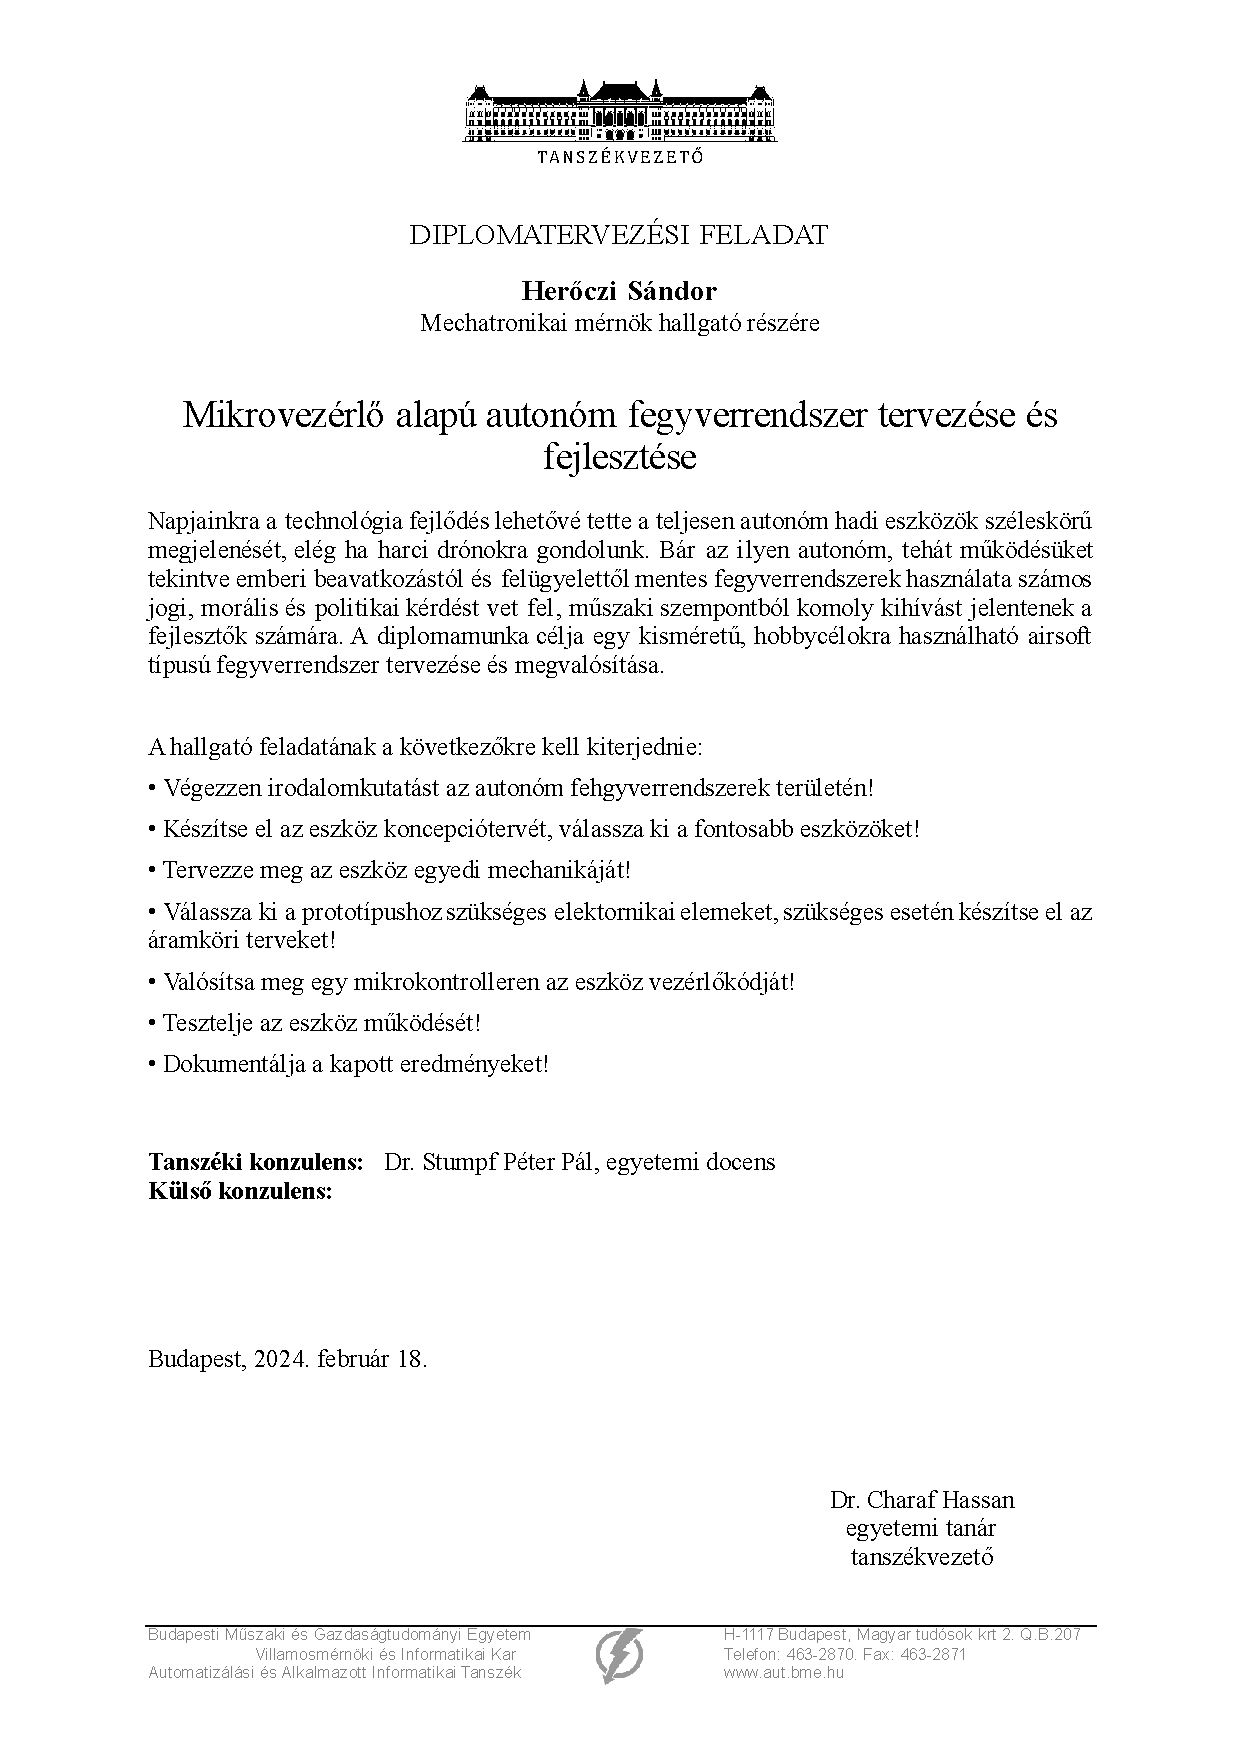
\includepdf[pages=-]{feladatkiiras.pdf}

\begin{titlepage}
	\begin{adjustwidth}{-2.5cm}{-2.5cm}

	
	\thispagestyle{empty}
	\centering

	\Large
	\rule{16cm}{1pt}\\
	\textsc{
		Budapesti Műszaki és Gazdaságtudományi Egyetem\\
		Villamosmérnöki és Informatikai Kar\\
		Automatizálási és Alkalmazott Informatikai Tanszék}\\[-0.3cm]
	\rule{16cm}{1pt}
	\end{adjustwidth}
	
	\vspace{2cm}
	
	\flushleft
	\Huge
	\textbf{\TITLE}
	
	\vspace{3cm}
	
	\Large
	\textbf{\AUTHOR}\\
	\NEPTUN\\
	
	\begin{tikzpicture}[overlay, remember picture]
		\node[anchor=center, xshift=5cm, yshift=-10cm] at (current page.center)
		{
\includegraphics[height=2cm]{autlogo}}; 
	\end{tikzpicture}
\end{titlepage}

\tableofcontents

\pagebreak

\section*{Hallgatói nyilatkozat}

Alulírott Herőczi Sándor, szigorló hallgató kijelentem, hogy ezt a diplomatervet meg nem engedett segítség nélkül, saját magam készítettem, csak a megadott forrásokat (szakirodalom, eszközök stb.) használtam fel. Minden olyan részt, melyet szó szerint, vagy azonos értelemben, de átfogalmazva más forrásból átvettem, egyértelműen, a forrás megadásával megjelöltem.\\

Hozzájárulok, hogy a jelen munkám alapadatait (szerző(k), cím, angol és magyar nyelvű tartalmi kivonat, készítés éve, konzulens(ek) neve) a BME VIK nyilvánosan hozzáférhető elektronikus formában, a munka teljes szövegét pedig az egyetem belső hálózatán keresztül (vagy hitelesített felhasználók számára) közzétegye. Kijelentem, hogy a benyújtott munka és annak elektronikus verziója megegyezik. Dékáni engedéllyel titkosított diplomatervek esetén a dolgozat szövege csak 3 év eltelte után válik hozzáférhetővé.\\

Kelt: \LOCATION, 2024.06.02.\\

\hfill
\begin{tabular}{c}
	........................................... \\
	Herőczi Sándor \\
\end{tabular}

\pagebreak


\section{Bevezetés}

\subsection{Az automata fegyverrendszerekről}

\lettrine{M}{int} manapság az ipar minden területén, így a fegyveriparban is egyre nagyobb mértékű a digitalizáció és az automatizáció. Ennek ékes példája a távolról irányítható lőállások térnyerése, amelyeknek nagy előnye a fegyver és a tüzér egymástól való elkülönítése, aminek több előnye is van. Természetesen a legfontosabb és leginkább szembetűnő, hogy ezzel a módszerrel minimalizálható, vagy akár megszüntethető a saját embereink életének kockáztatása. Ezentúl olyan helyen is tudjuk használni ezeket az eszközöket, ahova egy tradicionális géppuskafészek telepítése nehézkes lenne, például mostoha természeti körülmények közé, egy torony tetejére, vagy akár egy hadihajó oldalára. Szintén egy nagy előny, hogy ezek az eszközök felszerelhetők több kezeléssegítő alegységgel, például hőkamerával vagy éjjellátóval. Majdnem minden, számottevő hadsereggel rendelkező országnak van saját fejlesztésű távirányított fegyverrendszere.\\


\begin{wrapfigure}{r}{0.45\textwidth}
	\centering
	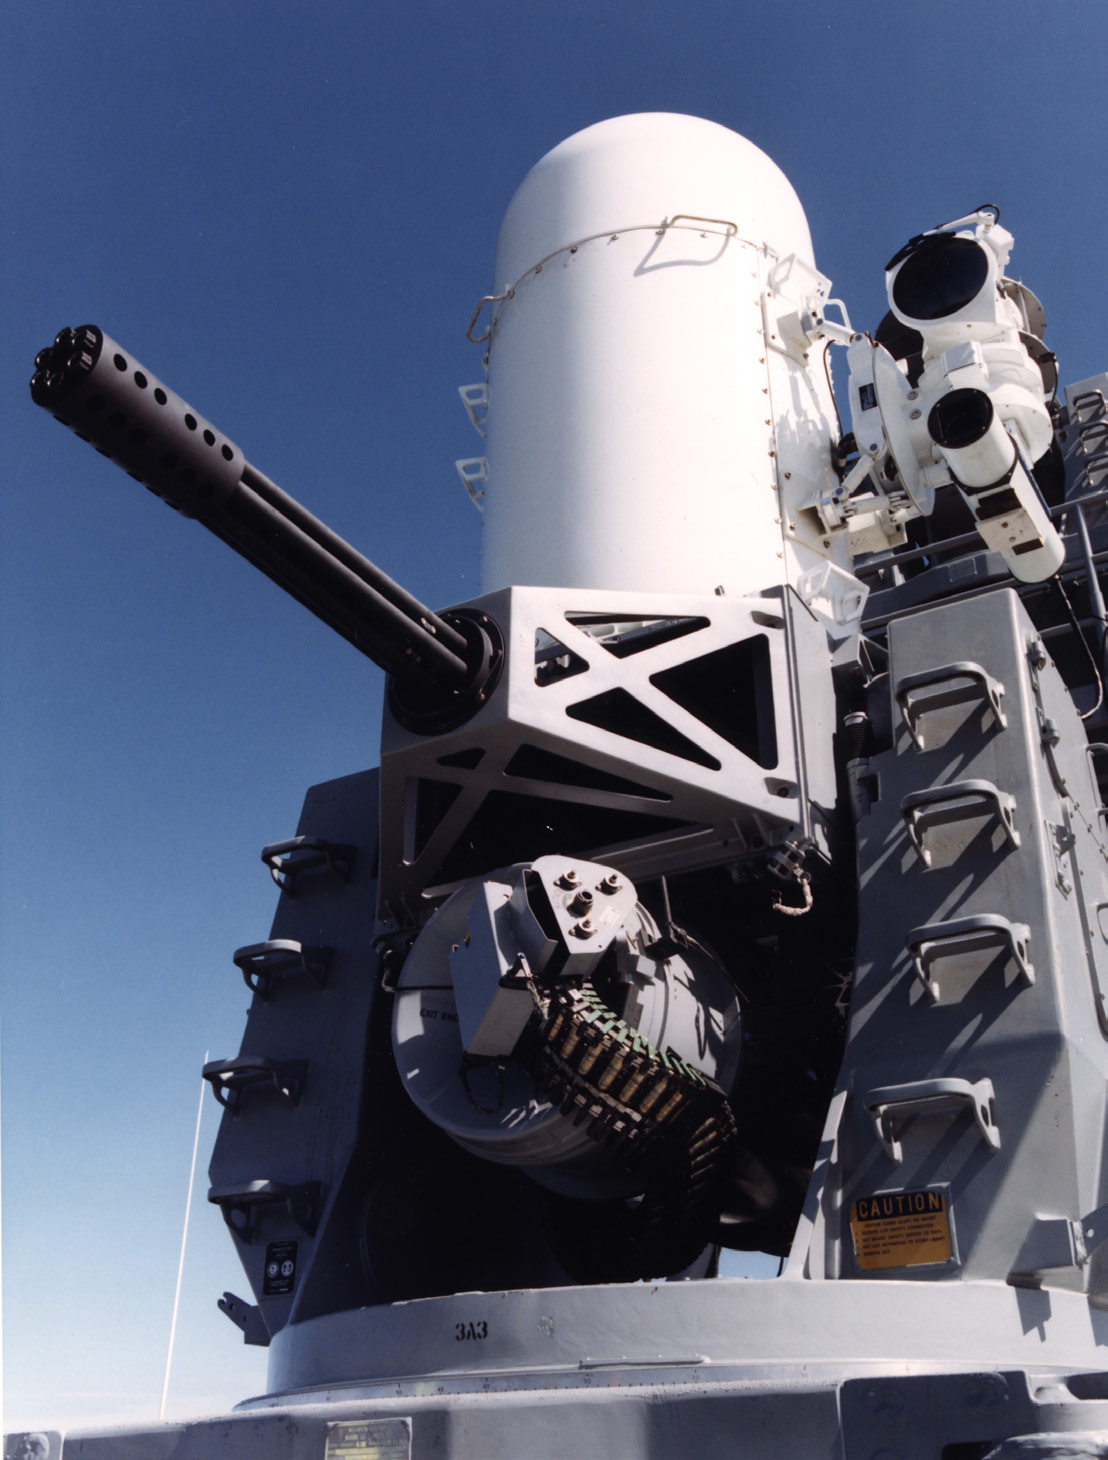
\includegraphics[width=0.95\linewidth]{irod_phalanx} 
	\caption{Phalanx CIWS rendszer}
	\label{fig:irod_phalanx}
\end{wrapfigure}

A következő lépés az automatizálás. Hiszen egyre erősebb hardverekkel rendelkezünk, egyre jobb algoritmusokat tudunk implementálni, és elértük az a szintet, hogy bizonyos helyzetekben a "gép" jobb munkát tud végezni, mint egy ember. Az első automatikus célzórendszerrel rendelkező légvédelmi gépágyú az amerikai \textsl{Phalanx CIWS} az 1970-es években került kifejlesztésre, ezzel megszületett a "Lethal autonomous weapon (LAW)" kifejezés.\\

A technológiát érthető módon leggyakrabban védelmi célokra használják, sokszor légvédelemre. A gyakorlatban nagy szerepe van Dél-Korea és Izrael védelmében, ahol a rakétatámadások mindennapos veszélyt jelentenek. Offenzív célokra a gyakorlatban még csak rakéták célzására használnak automatikát, a "terminátor" jellegű gyilkos robotok még csak fejlesztési fázisban vannak.

\subsection{Követelmények}\label{sec:kov}

A követelményeket egyrészt a később említett irodalomkutatás, másrészt pedig a saját ötleteim és a konzulensemmel való egyeztetés alapján alakítottam ki. Az "autonóm fegyverrendszer" alatt én egy olyan eszközt értek, ami egy pontban elhelyezve képes a környezetében felismerni a betanított célpontot, és arra tüzelni. Erre jó fikciós példa a \textsl{Portal} című játékban található \textsl{Sentry turret}, amely a \ref{portalsentry}. ábrán látható. Természetesen a konstrukciós tervezéshez nem ezt vettem alapul, de a működési elvhez adhat jó ötleteket akkor is, ha csak fikció. \\

\begin{wrapfigure}{r}{0.45\textwidth}
	\centering
	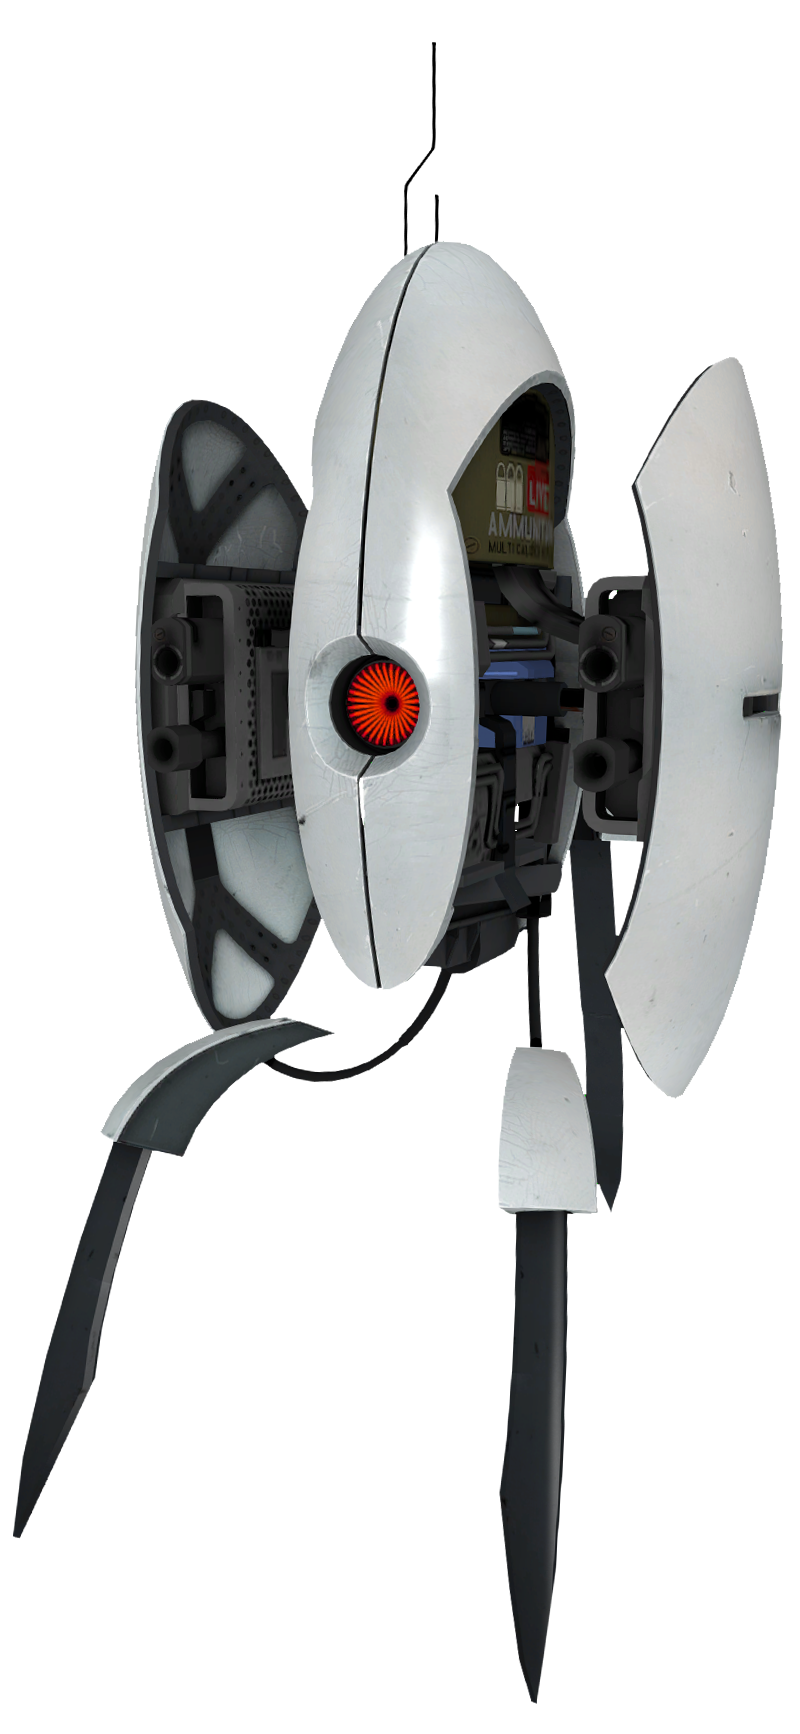
\includegraphics[width=0.8\linewidth]{portalsentry}
	\caption{Sentry Turret}
	\label{portalsentry}
\end{wrapfigure}

Szeretném a rendszert úgy megvalósítani, hogy a célfelismerés és tüzelést lehessen vezérelni "kézi vezérléssel", ahogy a valós katonai rendszerek többsége működik, illetve egy teljesen automatikus gépi látás algoritmussal. Automata működés során is talán az lenne a legéletszerűbb, hogy a célpont megtalálása és becélzása lenne automatikus, a tüzelés pedig emberi engedélyezést igényel, ezzel egy fokkal morálisabbá téve a projektet.\\

A hatásos távolságot én 10m-ben határoztam meg. Ezen a távolságon fel kell ismernie és el kell találnia egy 30x30 cm-es célpontot. Ezentúl szeretném, ha le tudná követni a 10 km/h-val futó ember mozgását. Ezek a határértékek a konstrukció tervezésénél fontos szempontok lesznek, tehát a későbbi fejezetekben számolok velük.\\


\pagebreak


\subsection{Irodalomkutatás}
A legjelentősebb katonai hatalmak mindegyike rendelkezik távvezérelt fegyverrendszerekkel, leggyakrabban valamilyen távolról irányított gépfegyver formájában. Azonban se az egyes országok nemzetbiztonságának, se a fegyveripari partnercégeknek nem áll érdekében a szükségesnél több információt kiadni. Ez egy kicsit megnehezítette az irodalomkutatást, de a képek alapján azért sok információt ki lehet nyerni.

\subsubsection{Valós rendszerek} \label{sec:valos}

\paragraph{CROWS \cite{crows}}
Az egyik legnagyobb darabszámban gyártott távirányított fegyverrendszer az amerikai \textsl{CROWS} rendszer, amely a NATO-országokban, köztük Magyarországon is rendszeresített. Ennek értelmében telepíthető sok NATO által használt páncélozott járműre, köztük a Humvee-ra, a Stryker-re, és a Buffalo MRAP-re. Több verziója létezik több kaliberrel, a \ref{fig:irod_crows}. ábrán egy M240B géppuskával látható.\\

\begin{figure}[h!]
	\centering
	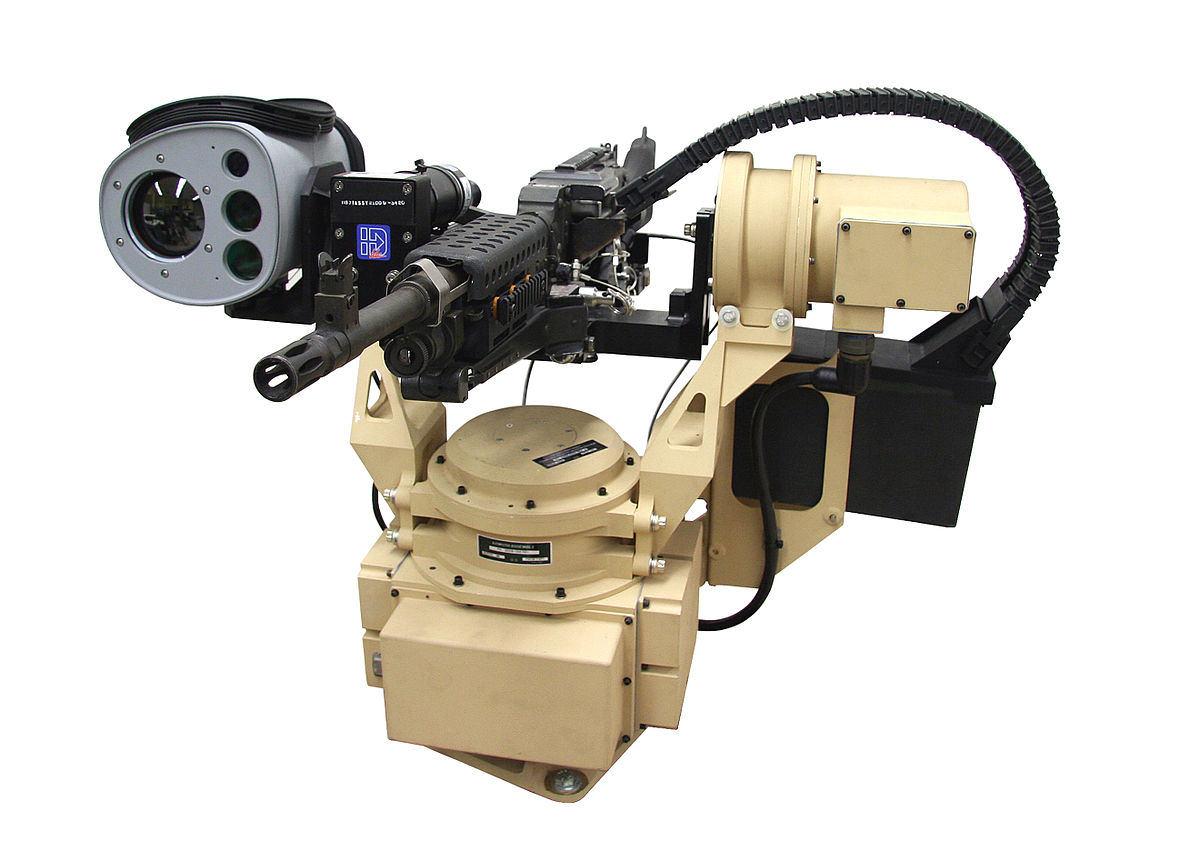
\includegraphics[width=1\linewidth]{irod_crows}
	\caption{Az amerikai CROWS rendszer}
	\label{fig:irod_crows}
\end{figure}

A szerelék a fegyverrel együtt $360^\circ$-ban képes elfordulni, és $-20^{\circ}$-tól $+60^{\circ}$-ig tud billenni. A fegyvercső giroszkóppal stabilizált. A kezelő egy 15 hüvelykes kijelzőn tud célozni a fegyverrel. A rendszer a sima kamera mellett rendelkezik hőkamerával is, így éjszaka is használható. Mind a két kamera el van látva lézeres távolságmérővel, amivel rá lehet állni a célpontra, és a jármű mozgása közben is lehet azt követni. A kamerát és a fegyvert lehet külön is mozgatni, ami azért hasznos, mert anélkül lehet követni a gyanús alakok mozgását, hogy félelmet keltenénk az emberekben.

\paragraph{Arbalet-DM \cite{arbalet}}
A \textsl{CROWS} rendszer orosz megfelelője a hasonló kialakítású \textsl{Arbalet-DM} (\ref{fig:irod_arbalet}.ábra). Ennek a rendszernek az alapja a 12.7 mm-es KORD nehézgéppuska. Rendelkezik 4 gránátvetővel is, amelyek füstfüggöny felhúzására használható. A kamera és a fegyver elhelyezése, de még a lőszer pozíciója is teljesen hasonló az amerikai párjához.

\begin{figure}[h!]
	\centering
	\includegraphics[width=1\linewidth]{irod_arbalet}
	\caption{Az orosz Arbalet-DM rendszer}
	\label{fig:irod_arbalet}
\end{figure}

A rendszer $360^\circ$-ban képes elfordulni, és $-20^{\circ}$-tól $+70^{\circ}$-ig tud billenni, tehát egy kicsit nagyobb részt tud lefedni, mint a CROWS. A hatótáv nappal 2000 m, éjszaka 1500 m. Ez a rendszer is el van látva hőkamerával és lézeres távolságmérővel.

\paragraph{DeFNder \cite{arbalet}}
A következő megoldás a belga \textsl{DeFNder} termékcsalád, amelynek két tagja a \textsl{Light} és a \textsl{Medium}(\ref{fig:irod_defnder}. ábra). Értelem szerűen kettő közül az utóbbi az, amelyre nehezebb fegyverzetet lehet telepíteni. A függőleges tengelyen $360^\circ$-ban képes elfordulni 90 fok/másodperc sebességgel, a vízszintes tengelyen $-45^{\circ}$-tól $+75^{\circ}$-ig tud billenni, 60 fok/másodperc sebességgel. Opcionálisan ellátható infravörös- és hőkamerával a rossz látási körülmények esetére, valamint lézeres távolságmérővel a ballisztikai kompenzációhoz.
\begin{figure}[h!]
	\centering
	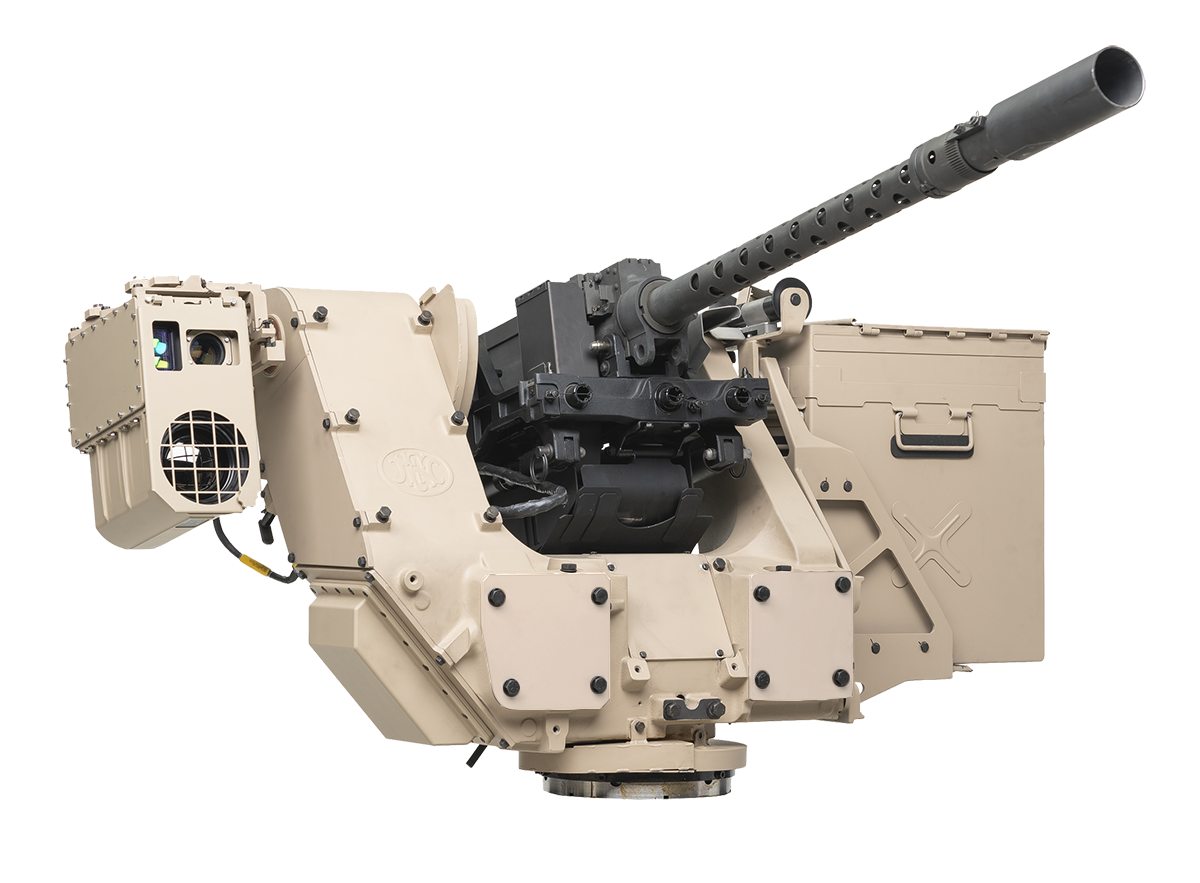
\includegraphics[width=1\linewidth]{irod_defnder}
	\caption{A belga DeFNder rendszer}
	\label{fig:irod_defnder}
\end{figure}


Elég sok közös vonást találtam a fentebb említett rendszerekben. Az elrendezésük nagyon hasonló, van egy függőleges forgástengely nagyjából a teljes rendszer súlypontján keresztül, valamint egy vízszintes forgástengely, nagyjából a fegyver csövével egy síkban. Erre valószínűleg azért van szükség, hogy a tüzelés során keletkező erők ne ébresszenek csavarónyomatékot a mozgató mechanizmuson. Az én esetemben nagy erők nem fognak ébredni, de a tervezési elvet érdemes követni.

\pagebreak

\subsubsection{Tüzelési mechanizmus}

A korábban említett rendszerek éles fegyverekkel vannak felszerelve, ami az én esetemben sajnos nem megvalósítható. Így valamilyen más megoldást kellett találni, ami legális, és megfelelően be lehet vele mutatni a célfelismerés és célzás működését. 


\paragraph{Paintball}

Több, a diplomamunkámhoz hasonló projektet is találtam, amelyek paintball puskákat használnak. Ezek a puskák sűrített levegőt alkalmaznak, hogy egy festékkel töltött golyót lőjenek ki. A torkolati sebességük nagyjából 280 fps, maximális hatékony távolságuk kb 25-30 m. Mivel a lövedék alakja gömb, és a cső sincs huzagolva, ezért nem túl pontos, főleg hosszú távon.\\

\begin{figure}[h!]
	\centering
	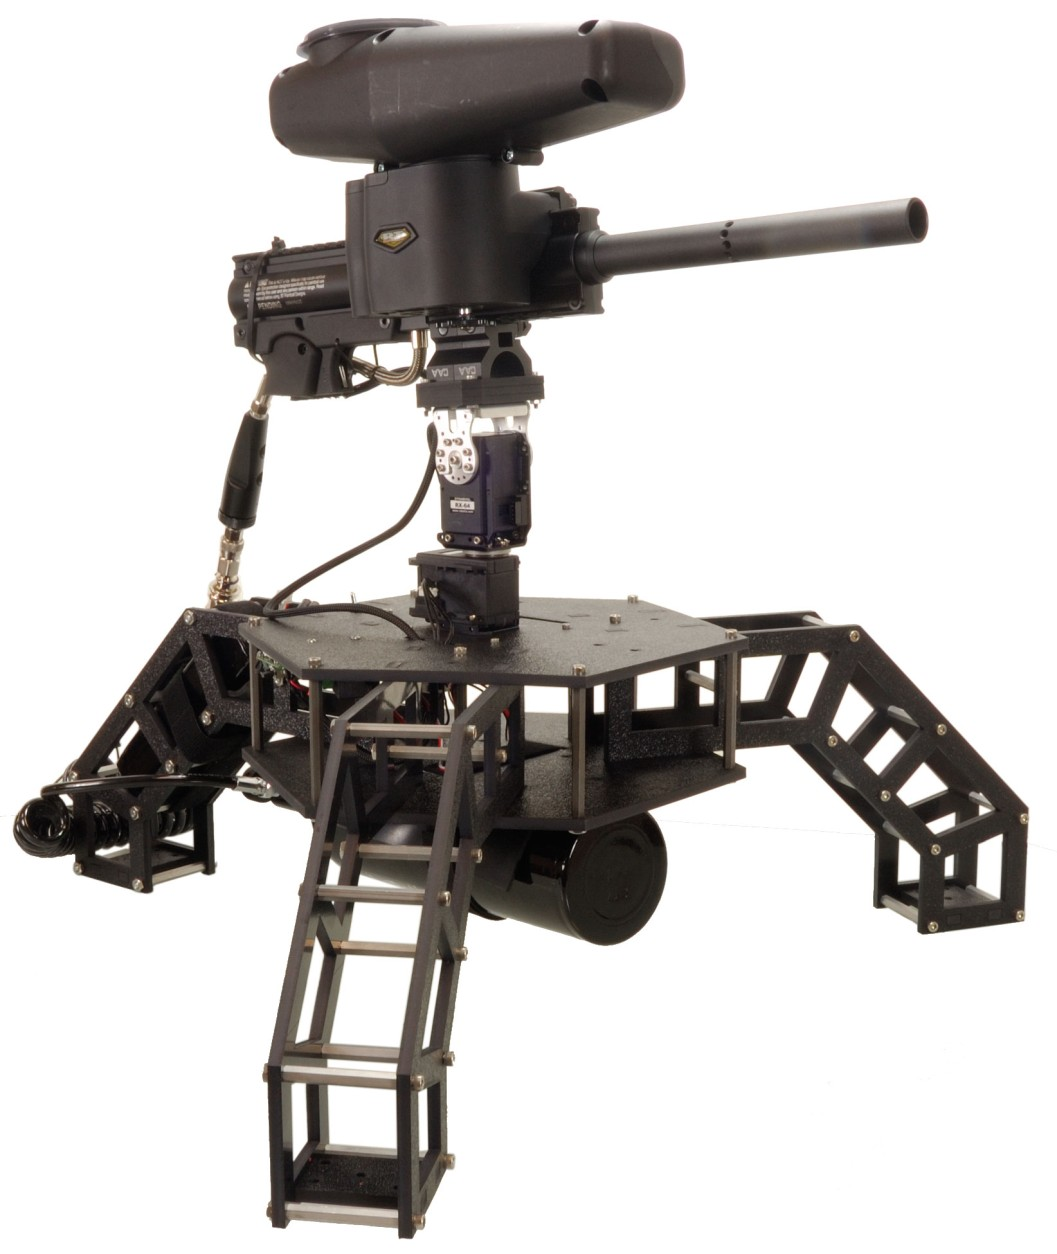
\includegraphics[width=0.6\linewidth]{irod_paintball}
	\caption{Paintball puska alapú rendszer}
	\label{fig:irod_paintball}
\end{figure}

További problémák, hogy a legolcsóbb paintball puska is 70000 Ft. fölött van, valamint a lövedék is viszonylag drága, és nem lehet újrahasznosítani. Ezentúl a fegyverek nagyok, nehezek, és ezért nehéz a beépítésük. 


\paragraph{Nerf}

A Nerf fegyverek a legelterjedtebb játékfegyverek. Sűrített levegővel lőnek ki egy hosszúkás szivacs lövedéket. A sűrített levegőt egy megfeszített rugó elengedésével érik el, amelyet vagy kézzel, vagy valamilyen áttételes villanymotorral húznak fel. A legjobb modellek torkolati sebessége 70 fps körül van, és kb. 15 m a hatótávolságuk. Ezen a távon viszonylag pontosak a lövedék kialakításából adódóan, de jelentős az esés, így a ballisztikai pályát komolyan kell venni. \\

Ezek a fegyverek modelltől függően 10000 Ft. - 40000 Ft. között mozognak, de a lövedékeket újra lehet használni. Az a probléma itt is fennáll, hogy nagy a fegyver teste, így nehezebb beépíteni. 

\paragraph{Airsoft}

Az airsoft fegyverek hasonló módon működnek, mint a Nerf puskák, de egy kisebb, műanyag golyót lőnek. Az elektromos airsoft fegyverek torkolati sebessége általában 300 fps és 400 fps között van, ami befolyásol a golyók tömege, a rugó minősége és rengeteg egyéb alkatrész. A hatótávjuk az átlagos fegyvereknek kb. 50 m, de fejlesztésekkel elérheti a 90 m-t is. A lövedék itt is golyó és a cső sincs huzagolva, mint a paintballnál, azonban az airsoft esetében használnak ún. hop-up kamrákat, amelyek perdületet adnak a golyónak.\\

Az airsoft fegyverek legnagyobb előnye a többi lehetőséggel szemben, hogy van egy kompakt egység, a "gearbox", ami felelős az elsütésért. Ezt ki lehet szedni egy fegyverből, vagy akár külön is meg lehet venni. Ez okkal nagyobb szabadságot ad a beépítéshez, és a végeredmény is sokkal kompaktabb lesz. Az elsütés is csak az áramkör zárását jelenti a gearboxban, ami egyszerűen vezérelhető a mikrokontrollerrel.



\section{Megvalósítás}

A \ref{sec:valos}. bekezdésben vizsgált rendszerek alapján körvonalazódott, milyen megoldást szeretnék én is alkalmazni. Nagyon leegyszerűsítve egy 360 fokban forgó toronyról lenne szó, aminek a tetején helyezkedik el a billenthető fegyverzet. Szemléltetésképpen készítettem a \ref{fig:megval_mockup}. ábrát. 

\begin{figure}[h!]
	\centering
	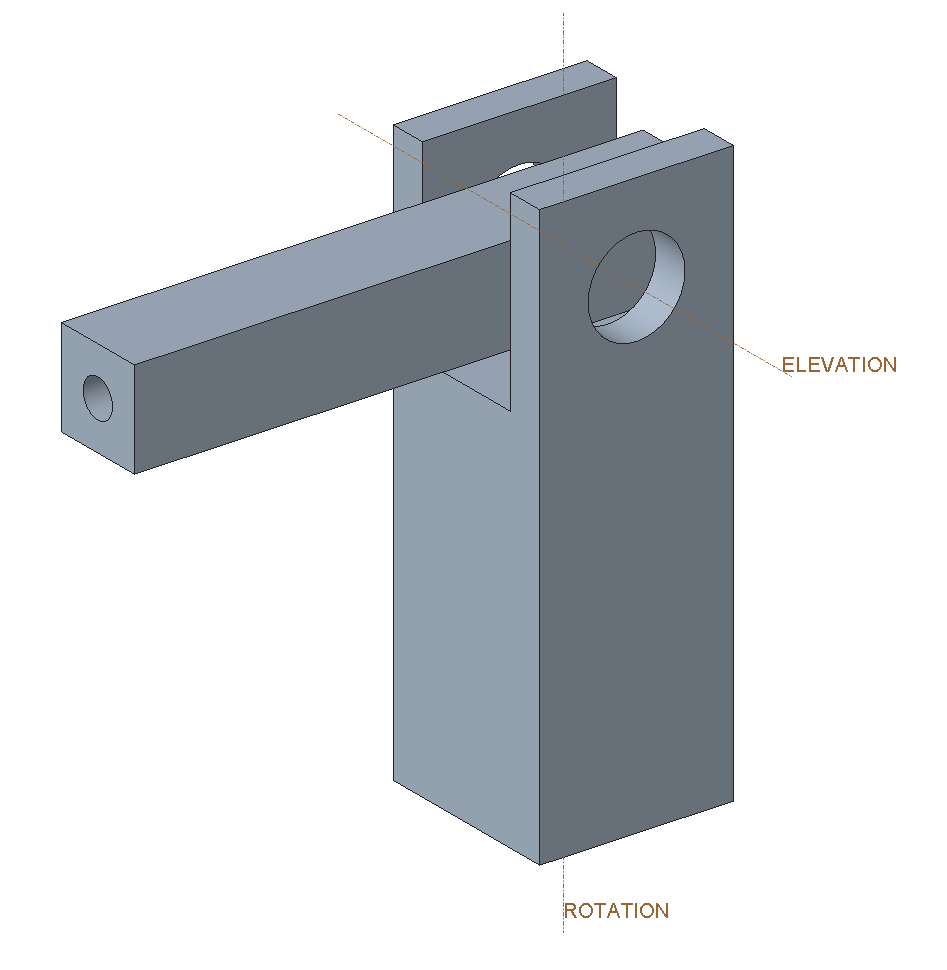
\includegraphics[width=0.6\linewidth]{mockup}
	\caption{A rendszerelrendezés}
	\label{fig:megval_mockup}
\end{figure}

Ki kellett számolnom bizonyos geometriai megkötéseket, amelyek szükségesek a tervezéshez, illetve az alkatrészek kiválasztásához. \\

A torony szükséges fordulatszámát a következőképpen lehet kiszámolni:


\begin{equation}
	rpm_{min} = \frac{v_t}{2 \cdot \pi \cdot r} = \frac{2.778 \w{m/s}}{2 \cdot \pi \cdot \w{m}} = 0.442 \w{1/s} = 26.526 \w{1/min}
\end{equation}

ahol:

\begin{tabular}{cl}
	$v\_t$ & A célpont sebessége a fegyvercsőre merőlegesen, \\
	$r$ & A távolság a célpont és a rendszer között\\
\end{tabular}

Meg lehet állapítani a torony mozgásának felbontását is, tehát hogy hány fokonként lehet állítani a mozgását.

\begin{equation}
	\alpha_{min} = \arcsin\left(\frac{a}{2 \cdot r}\right) \cdot 2 = \arcsin\left(\frac{0.3 \w{m}}{2 \cdot 10 \w{m}}\right) \cdot 2 = 1.719 {^\circ}
\end{equation}

ahol:

\begin{tabular}{cl}
	$a$ & A célpont mérete  \\
	$r$ & A távolság a célpont és a rendszer között\\
\end{tabular}






%\subsection{Motorok}
%
%A motorok kiválasztáshoz először a 
%
%
%\subsection{Hardver}
%
%A hardver tervezését először egy 
%

\subsubsection{Mikrovezérlő}

A mikrokontroller kiválasztásánál több opciót vizsgálta, többek között az {Arduino}, az \textsl{STM-32} és a \textsl{Raspberry PI} modelleket. Azonban ahogy összehasonlítottam a különböző opciókat, körvonalazódott, hogy a \textsl{Raspberry PI} lesz a megfelelő megoldás. A kamera illesztése különösen fontos a végtermék működése szempontjából, és ezen a területen magasan kiemelkedik a Raspberry a többi mikrovezérlő közül, mivel magán a gyártó a termékcsaládon belül ajánl több kamera modult, amik illesztése már kiforrott az összes Raspberry-hez.\\

Ezentúl a \textsl{Raspberry PI} erősebb, mint a fentebb említett mikrokontrollerek. Linux rendszert futtat, és lehet rajta Python nyelven programozni, ami gépi látás, automatizálás projekteknél hatalmas előny. Számos ki-és bemenete van, ráadásul támogatja a \textsl{Bluetooth}, \textsl{Wi-Fi}, és \textsl{Ethernet} kapcsolatokat is, nem beszélve a rengeteg bővítő "kabátról", amiket lehet kapni hozzá. Ezek a termék továbbfejlesztését nagyban könnyítik, ráadásul kevesebb munkát kell a nyomtatott áramkör tervezésébe tenni.


\subsubsection{Elsütő mechanizmus}
Az elsütő mechanizmusnak egy \textsl{Specna Arms M4}-ből kiszerelt gearbox-ot, illetve csövet használtam. A gearbox-on belül kellett alakítanom a működésen, hogy megfelelően bele lehessen illeszteni a rendszerbe. Az elsütőbillentyűt, a tűzkapcsolót és minden ehhez tartozó mechanikai elemet kiszereltem, illetve áthuzaloztam. Erre azért volt szükség, mert különben csak a ravasz meghúzásával lehetett volna tüzelni, ami bonyolít a rendszer megvalósításán. A gearbox belső kialakítása a \ref{fig:gearboxbele}. ábrán látható.

\begin{figure}[h!]
	\centering
	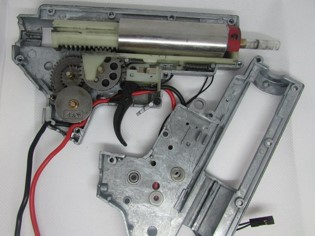
\includegraphics[width=0.6\linewidth]{gearboxbele}
	\caption{A gearbox belseje}
	\label{fig:gearboxbele}
\end{figure}

A fegyver gearbox-ot körülvevő alkatrészeiről le tudtam venni méreteket, ez alapján alakítottam ki később a 3D nyomtatott alkatrészeket. Így végeredményben egy magába zárt alkatrészem lett, amin habár mechanikus nem lehet állítani a tüzelés módját, de csupán két vezetékkel csatlakozik az elektronikához. 



%\subsubsection{Motorok}
%
%\subsubsection{Vezérlő áramkör}
%
%
%\subsection{Gépészeti tervezés}
%
%\subsection{Szoftver}


























\pagebreak
	\begin{thebibliography}{}
	\bibitem{crows}
	Leírás a CROWS rendszerről \hfill (Hozzáférés: 2024.01.22.) \\
	{\footnotesize \url{https://www.globalsecurity.org/military/systems/ground/m101-crows.htm}},
	\bibitem{arbalet}
	Leírás az Arbalet-DM rendszerről \hfill (Hozzáférés: 2024.01.22.) \\
	{\footnotesize \url{http://roe.ru/eng/catalog/land-forces/RWS/arbalet-dm/}},
	\bibitem{arbalet}
	Leírás az deFNder Medium rendszerről \hfill (Hozzáférés: 2024.01.22.) \\
	{\footnotesize \url{https://fnamerica.com/products/weapon-systems/defnder-medium/}},


\end{thebibliography}


\end{document}